\subsection{Out of Order and Speculative Execution}
\label{sec:out_of_order}

CPU cores can execute instructions orders of magnitude faster than DRAM can
read data. CPU architects attempt to bridge this gap by using hyper-threading
(\S~\ref{sec:cpu_die}), caching (\S~\ref{sec:caching}), and out of order and
speculative execution. Out of order execution can safely be ignored when
developing a general understanding of SGX, but becomes necessary when
understanding implementation details. Out of order and speculative execution
can also introduce noise in the data obtained from cache timing attacks. This
section provides an overview of out of order and speculative execution that is
sufficient for reasoning about SGX and cache timing attacks.
\cite{patterson2013architecture} and \cite{hennessy2012architecture} cover the
concepts in great depth, while Intel's optimization manual
\cite{intel2014optimization} provides details specific to Intel CPUs.

% The Haswell Microarchitecture: Optimization S 2.1

Figure~\ref{fig:cpu_out_of_order} provides a more detailed view of the CPU core
components involved in out of order execution, and omits some less relevant
details from Figure~\ref{fig:cpu_core}.

\begin{figure}[hbt]
  \center{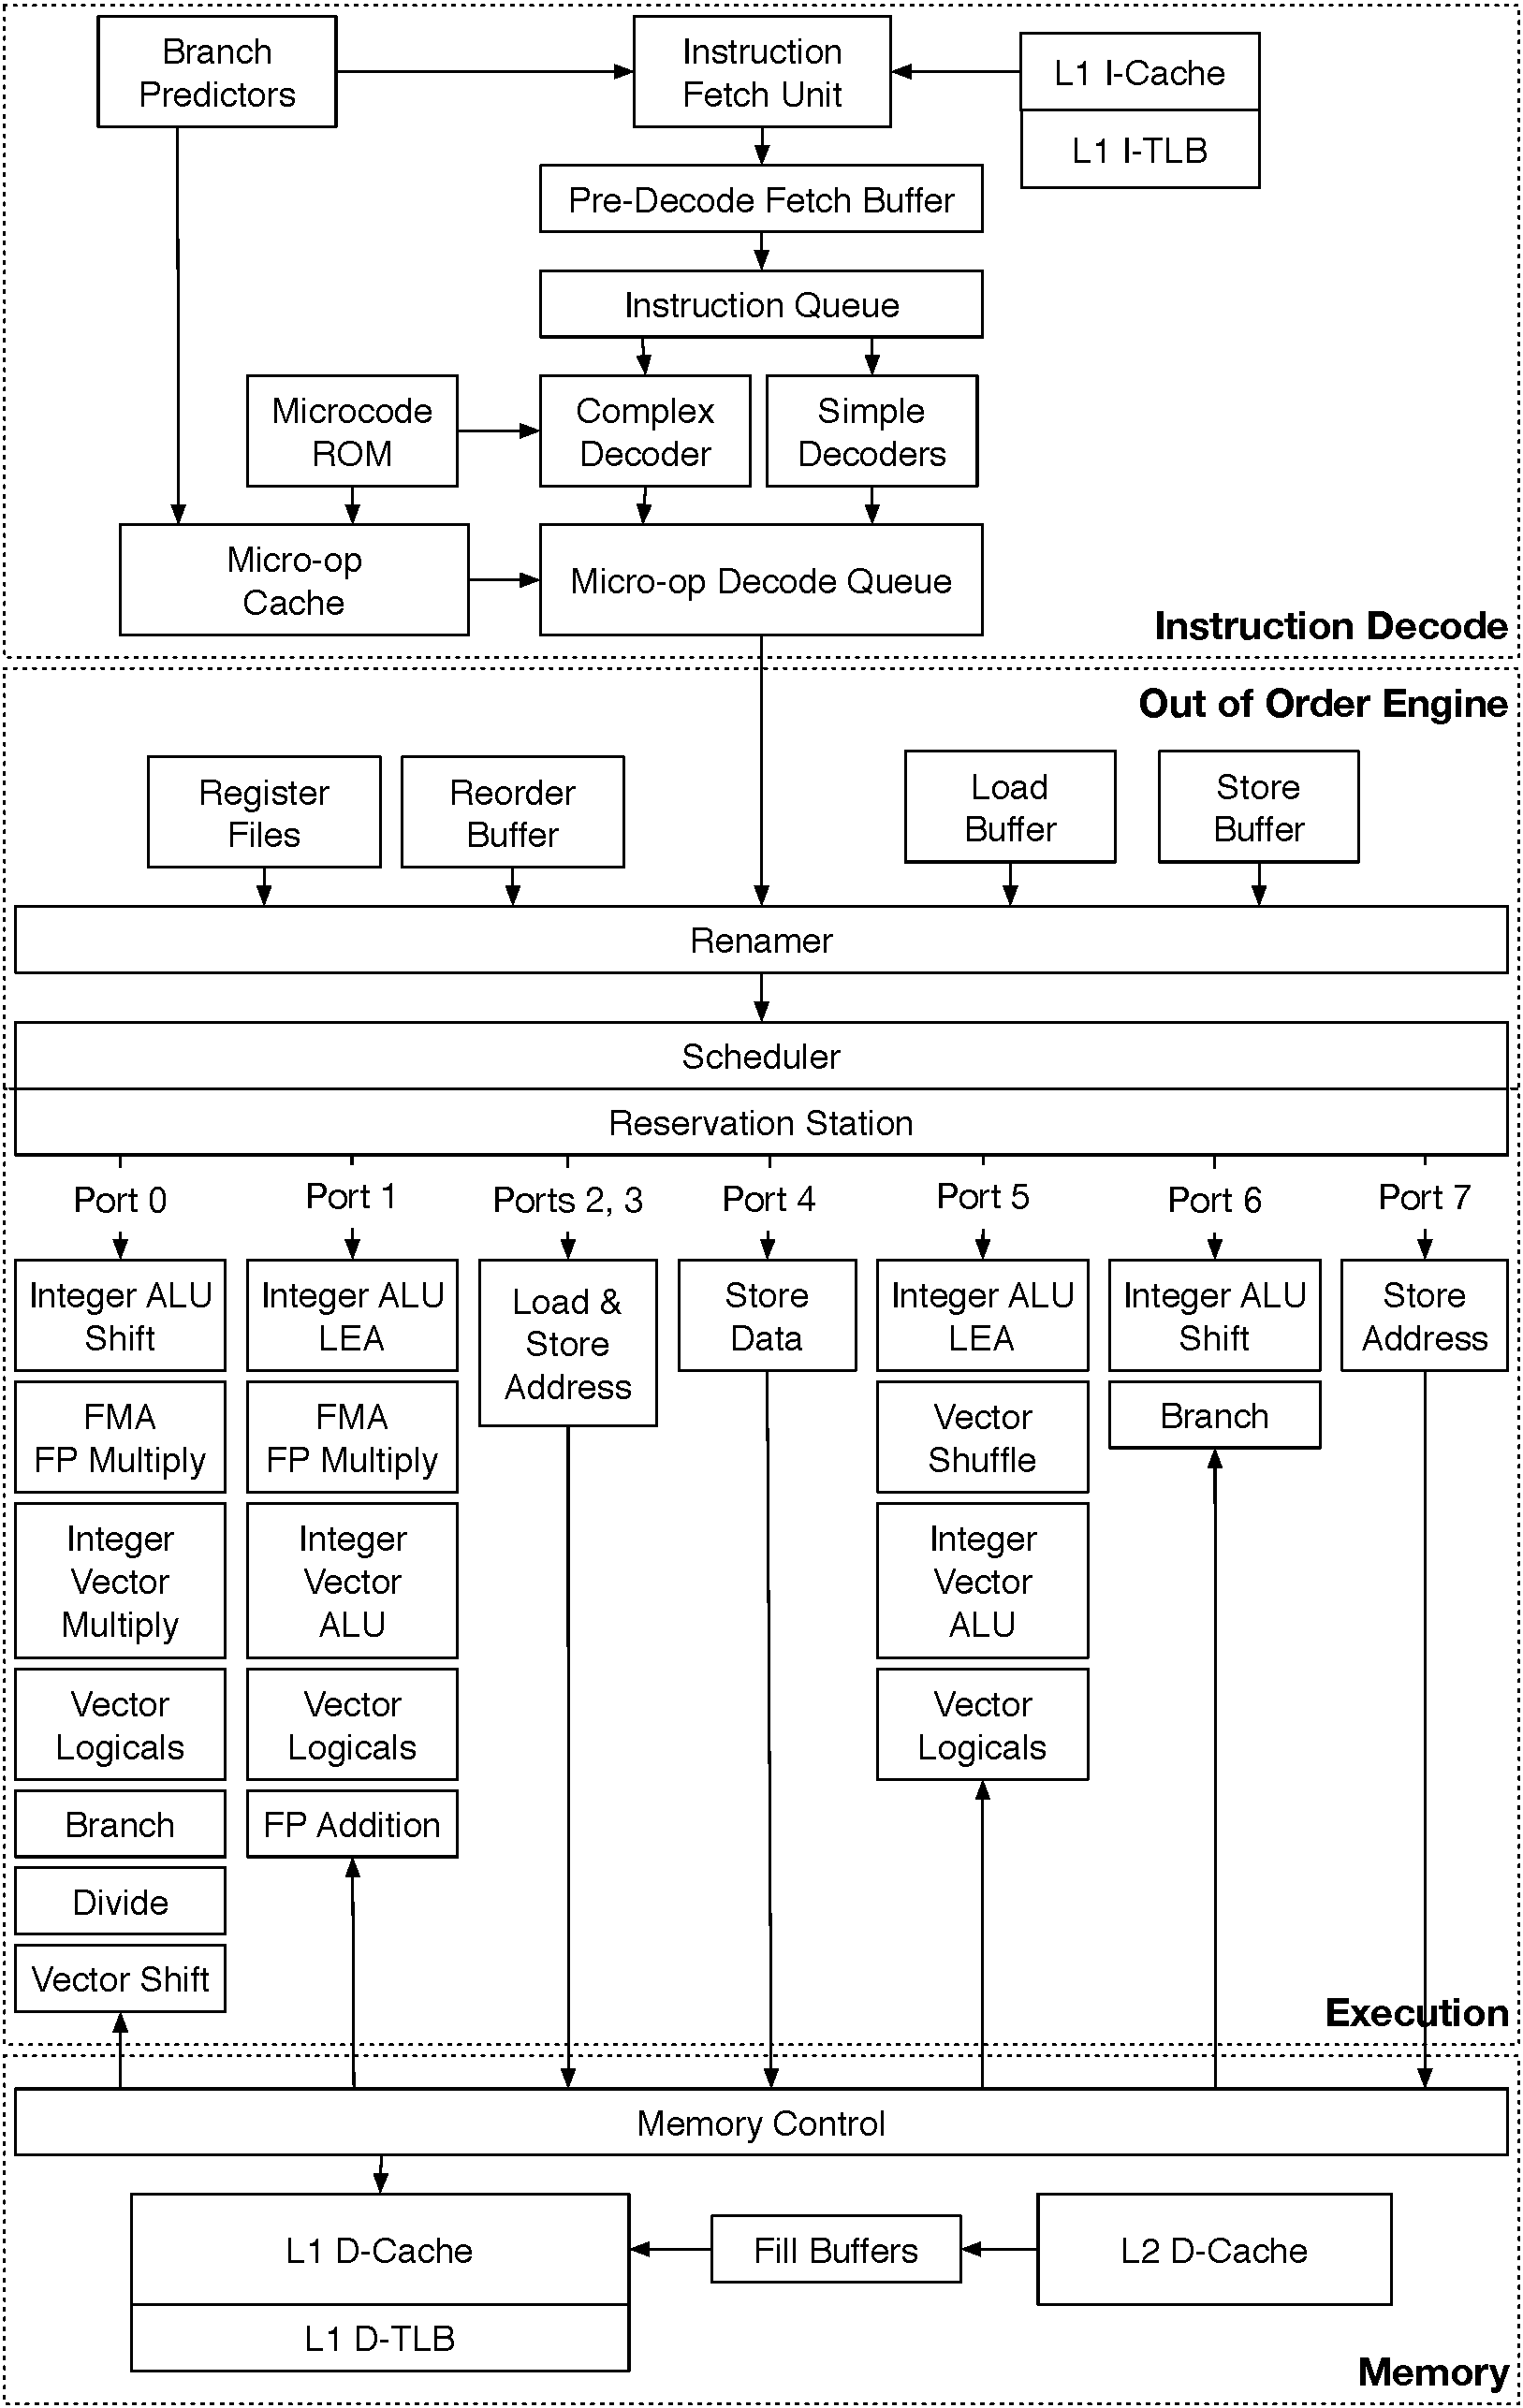
\includegraphics[width=85mm]{figures/cpu_out_of_order.pdf}}
  \caption{
    The structures in a CPU core that are relevant to out of order and
    speculative execution. Instructions are decoded into micro-ops, which are
    scheduled on one of the execution unit's ports. The branch predictor
    enables speculative execution when a branch is encountered.
  }
  \label{fig:cpu_out_of_order}
\end{figure}

% Intel Microarchitecture Code Name Sandy Bridge Pipeline Overview:
%     Optimization S 2.2.1
% The Front End: Optimization S 2.2.2

The Intel architecture defines a \textit{complex instruction set} (CISC).
However, virtually all modern CPUs are architected following \textit{reduced
instruction set} (RISC) principles. This is accomplished by having the
instruction decode stages break down each instruction into \textit{micro-ops},
which resemble RISC instructions. The other stages of the execution pipeline
work exclusively with micro-ops.


\subsubsection{Out of Order Execution}

% Out of Order Engine: Optimization S 2.2.23
% The Execution Core: S 2.2.4

Different types of instructions require different logic circuits, called
\textit{functional units}. For example, the arithmetic logic unit (ALU), which
performs arithmetic operations, is completely different from the load store
unit, which peforms memory operations. Different circuits can be used at the
same time, so each CPU core can execute multiple micro-ops in parallel.

The core's out of order engine receives decoded micro-ops, and identifies the
micro-ops that can execute in parallel, assigns them to functional units, and
combines the outputs of the units so that the results are equivalent to having
the micro-ops executed sequentially in the order in which they come from the
decode stages.

For example, consider the sequence of pseudo micro-ops\footnote{The set of
micro-ops used by Intel CPUs is not publicly documented. The ficticious
examples in this section suffice for illustration purposes.} in
Table~\ref{fig:out_of_order_micro_ops} below. The \texttt{OR} uses the result
oh the \texttt{LOAD}, but the \texttt{ADD} does not. Therefore, a good
scheduler can assign the \texttt{LOAD} to the load store unit and the
\texttt{ADD} to the ALU, in the same cycle.

\begin{table}[hbt]
  \center{\begin{tabular}{| l | l | l |}
  \hline
  \textbf{\#} & \textbf{Micro-op} & \textbf{Meaning}\\
  \hline
  1 & \texttt{LOAD RAX, RSI} & RAX $\leftarrow$ DRAM[RSI]\\
  \hline
  2 & \texttt{OR RDI, RDI, RAX} & RDI $\leftarrow$ RDI $\lor$ RAX\\
  \hline
  3 & \texttt{ADD RSI, RSI, RCX} & RSI $\leftarrow$ RSI + RCX\\
  \hline
  4 & \texttt{SUB RBX, RSI, RDX} & RBX $\leftarrow$ RSI - RDX\\
  \hline
  \end{tabular}}
  \caption{
    Pseudo micro-ops for the out of order execution example.
  }
  \label{fig:out_of_order_micro_ops}
\end{table}

% Renamer: Optimization S 2.2.3.1

The out of order engine in recent Intel CPUs works roughly as follows.
Micro-ops received from the decode queue are written into a \textit{reorder
buffer} (ROB) while they are \textit{in-flight} in the execution unit. The
\textit{register allocation table} (RAT) matches each register with the last
reorder buffer entry that updates it. The \textit{renamer} uses the RAT to
rewrite the source and destination fields of micro-ops as they are written in
the ROB, as illustrated in Tables \ref{fig:out_of_order_rob} and
\ref{fig:out_of_order_rat}. Note that the ROB representation makes it easy to
determine the dependencies between micro-ops.

\begin{table}[hbt]
  \center{\begin{tabular}{| l | l | l | l | l |}
  \hline
  \textbf{\#} & \textbf{Op} & \textbf{Source 1} & \textbf{Source 2} & \textbf{Destination}\\
  \hline
  1 & LOAD & RSI & $\emptyset$ & RAX \\
  \hline
  2 & OR & RDI & ROB \#1 & RSI \\
  \hline
  3 & ADD & RSI & RCX & RSI \\
  \hline
  4 & SUB & ROB \# 3 & RDX & RBX \\
  \hline
  \end{tabular}}
  \caption{
    Data written by the renamer into the reorder buffer (ROB), for the
    micro-ops in Table~\ref{fig:out_of_order_micro_ops}.
  }
  \label{fig:out_of_order_rob}
\end{table}

\begin{table}[hbt]
  \center{\begin{tabular}{| l | r | r | r | r | r | r |}
  \hline
  \textbf{Register} & RAX & RBX & RCX & RDX & RSI & RDI \\
  \hline
  \textbf{ROB \#} & \#1 & \#4 & $\emptyset$ & $\emptyset$ & \#3 & \#2 \\
  \hline
  \end{tabular}}
  \caption{
    Relevant entries of the register allocation table after the micro-ops in
    Table~\ref{fig:out_of_order_micro_ops} are inserted into the ROB.
  }
  \label{fig:out_of_order_rat}
\end{table}

% Scheduler: Optimization S 2.2.3.2

The scheduler decides which micro-ops in the ROB get executed, and places them
in the \textit{reservation station}. The reservation station has one port
for each functional unit that can execute micro-ops independently. Each
reservation station port port holds one micro-op from the ROB. The reservation
station port waits until the micro-op's dependencies are satisfied and forwards
the micro-op to the functional unit. When the functional unit completes
executing the micro-op, its result is \textit{written back} to the ROB, and
forwarded to any other reservation station port that depends on it.

The ROB stores the results of completed micro-ops until they are
\textit{retired}, meaning that the results are \textit{committed} to the
register file and the micro-ops are removed from the ROB. Although micro-ops
can be executed out of order, they must be retired in program order, in order
to handle exceptions correctly. If micro-op causes a hardware exception
(\S~\ref{sec:faults}), all the following micro-ops in the ROB are
\textit{squashed}, and their results are discarded.

In the example above, the \texttt{ADD} can complete before the \texttt{LOAD},
because it does not require a memory access. However, the \textit{ADD}'s result
cannot be committed before \texttt{LOAD} completes. Otherwise, if the
\textit{ADD} is committed and the \textit{LOAD} causes a page fault, software
will observe an incorrect value for the  RSI register.

% Load and Store Operation Overview: Optimization S 2.2.5

The ROB is tailored for discovering register dependencies between micro-ops.
However, micro-ops that execute out of order can also have memory dependencies.
For this reason, out of order engines have a \textit{load buffer} and a
\textit{store buffer} that keep track of in-flight memory operations and are
used to resolve memory dependencies.

Out of order execution can introduce noise in cache timing attacks. First,
memory accesses may not be performed in program order, which can impact the
lines selected by the cache eviction algorithms. Second, out of order execution
may result in cache fills that do not correspond to executed instructions. For
example, a load that follows a faulting instruction may be scheduled and
executed before the fault is detected.


\subsubsection{Speculative Execution}

% Branch Prediction: Optimization S 2.2.2.3

Branch instructions, also called \textit{branches} change the instruction
pointer (RIP, \S~\ref{sec:registers}), if a condition is met (\textit{the
branch is taken}). They are used to compile \texttt{if}-style conditional
statements and in looping statements such as \texttt{while} and \texttt{for}.
The most well-known branching instructions in the Intel architecture are in the
\texttt{j\textit{cc}} family, such as \texttt{je} (jump if equal).

Branches pose a challenge to the decode stage, because the instruction that
should be fetched after a branch is not known until the branching condition is
evaluated. In order to avoid stalling the decode stage, modern CPU designes
include \textit{branch predictors} that use historical information to guess
whether a branch will be taken or not.

When a branch instruction is encountered in the decode stage, it asks the
branch predictor for a guess as to whether the branch will be taken or not. The
decode stage bundles the branch condition and the predictor's guess into a
branch check micro-op, and then continues decoding on the path indicated by the
predictor. The micro-ops following the branch check are marked as
\textit{speculative}.

When the branch check micro-op is executed, the branch unit checks whether the
branch predictor's guess was correct. If that is the case, the branch check is
retired successfully. The scheduler handles \textit{mis-predictions} by
squashing all the micro-ops following the branch check, and by signaling the
instruction decoder to flush the micro-op decode queue and start fetching the
instructions that follow the correct branch.

Speculative execution needs to be accounted for in cache timing attacks, as
mis-predicted speculative memory accesses can still cause cache fills.
Therefore, the attacker may observe cache fills that don't correspond to
instructions that were actually executed by the victim software.

% Data Prefetching: Optimization S 2.2.5.4

Modern CPUs also attempt to predict memory read patterns, so they can
\textit{prefetch} the memory locations that are about to be read into the
cache. Prefetching minimizes the latency of succesfully predicted read
operations, as their data will already be cached. This is accomplished by
exposing circuits called prefetchers to memory accesses and cache misses. Each
prefetcher can recognize a particular access pattern, such as squentially
reading an array's elements. When memory accesses match the pattern that a
prefetcher was built to recognize, the prefetcher loads the cache line
corresponding to the next memory access in its pattern.

Prefetching introduces noise in cache timing attacks, as the attacker may
observe cache fills that don't correspond to instructions in the victim code,
even when accounting for speculative execution.
